\documentclass[11pt]{article}

\usepackage{amsmath}
\usepackage{amssymb}
\usepackage{fancyhdr}
\usepackage{isotope}
\usepackage{graphicx}
\graphicspath{{./images/}{./}}
\usepackage{array}
\usepackage{caption}
\usepackage{subcaption}

\oddsidemargin0cm
\topmargin-2cm     %I recommend adding these three lines to increase the 
\textwidth16.5cm   %amount of usable space on the page (and save trees)
\textheight23.5cm  

\newcommand{\question}[2] {\vspace{.25in} \hrule\vspace{0.5em}
\noindent{\bf #1: #2} \vspace{0.5em}
\hrule \vspace{.10in}}
\renewcommand{\part}[1] {\vspace{.10in} {\bf (#1)}}

\newcommand{\myname}{Matthew J. Urffer}
\newcommand{\myemail}{murffer@utk.edu}
\newcommand{\myhwnum}{3}

\pagestyle{fancyplain}
\lhead{\fancyplain{}{\textbf{HW\myhwnum}}}      % Note the different brackets!
\rhead{\fancyplain{}{\myname\\ \myemail}}
\chead{\fancyplain{}{CHEM-630}}

\begin{document}

\medskip                        % Skip a "medium" amount of space
                                % (latex determines what medium is)
                                % Also try: \bigskip, \littleskip

\thispagestyle{plain}
\begin{center}                  % Center the following lines
{\Large CHEM-630 Assignment \myhwnum} \\
\myname \\
\myemail \\
January 22, 2013 \\
\end{center}

\question{1.11}{Atoms}

%%%%%%%%%%%%%%%%%%%%%%%%%%%%%%%%%%%%%%%%%%%%%%%%%%%%%%%
\part{a}{Calculate the average atomic weight of the element when Ag has 51.35\% \isotope[107]{Ag} and \isotope[109]{Ag}}


%%%%%%%%%%%%%%%%%%%%%%%%%%%%%%%%%%%%%%%%%%%%%%%%%%%%%%%
\part{b}{Identify an element which has 7 stable isotopes}
{Calculate the nuclear radius of \isotope[242]{Cr}}

An approximation of the nuclear radius is given by \ref{eqn:NuclearRadius}
\begin{align}
	r(A)[cm] = 1.4\times10^{-13}A^{1/3} 
	\label{eqn:NuclearRadius}
\end{align}
\isotope[242]{Cr} has an $A=242$, yielding
\begin{align}
	r(A=242)[cm] &= 1.4\times10^{-13}242^{1/3} 
					 &= 8.7\times10^{-13} cm 
\end{align}
The nuclear radius listed on Wolfram-Alpha for Cr was 3.4 fm, which is roughly one half of the calculated radius.

%%%%%%%%%%%%%%%%%%%%%%%%%%%%%%%%%%%%%%%%%%%%%%%%%%%%%%%
\part{c}{Calculate the nuclear mass of \isotope[27]{Mg}}

The atomic mass of \isotope[27]{Mg} is 26.98434 u. Mg has 12 protons, and therefore a neutral isotope would have 12 electrons.
The nuclear mass is then
\begin{align}
	M(27,12) &= 26.98434 u - (12e^-)\frac{5.4858\times10{-4} u}{e^-}
				&= 26.9778 u
\end{align}

%%%%%%%%%%%%%%%%%%%%%%%%%%%%%%%%%%%%%%%%%%%%%%%%%%%%%%%
\part{d}{Look up the mass in mu of \isotope[19]{O}. Then add the masses of the constituent particles. Explain why there is a discrepancy}

The atomic mass of \isotope[19]{O} is 19.00358 u (Wolfram-Alpha).
The masses of the constituents are:
\begin{center}
	\begin{tabular}{c c c}
	Constituent & Amount & Mass \\
	\hline
	\hline
	Neutrons & 11 & 11.0953 \\
	Protons & 8 & 8.0582 \\
	Electrons & 8 & 0.0044 \\ 
	\multicolumn{2}{c}{Total} & 19.1579
\end{tabular}
\end{center}
The difference in the total mass of the constituents and the atomic mass comes is 0.1543 u, which comes from the binding energy.
The act of bringing the nucleus together creates a nuclear potential well, and the excess mass is turned into the energy depth of this potential well.

%%%%%%%%%%%%%%%%%%%%%%%%%%%%%%%%%%%%%%%%%%%%%%%%%%%%%%%
\part{e}{Calculate the binding energy per nucleon of \isotope[45]{Sc}}

The semi-empirical equation for the binding energies was implemented in MATLAB. For \isotope[45]{Sc} the total binding energy was calculated to be 389.1 MeV, and with 45 nucleons the binding energy per nucleon is then 8.647 MeV. The published value by the NNDC (BNL) is 8.618 MeV per nucleon.

%%%%%%%%%%%%%%%%%%%%%%%%%%%%%%%%%%%%%%%%%%%%%%%%%%%%%%%
\part{f}{Draw three isotopes with Z = 45}

Isotopes are nuclides with the same Z (number of protons), but have a different number of neutrons.
The isotopes of Z=45 are shown in Figure ~\ref{fig:Isotopes}.
\begin{figure*}[!ht]
	\centering
	\begin{subfigure}[b]{0.3\textwidth}
		\centering
		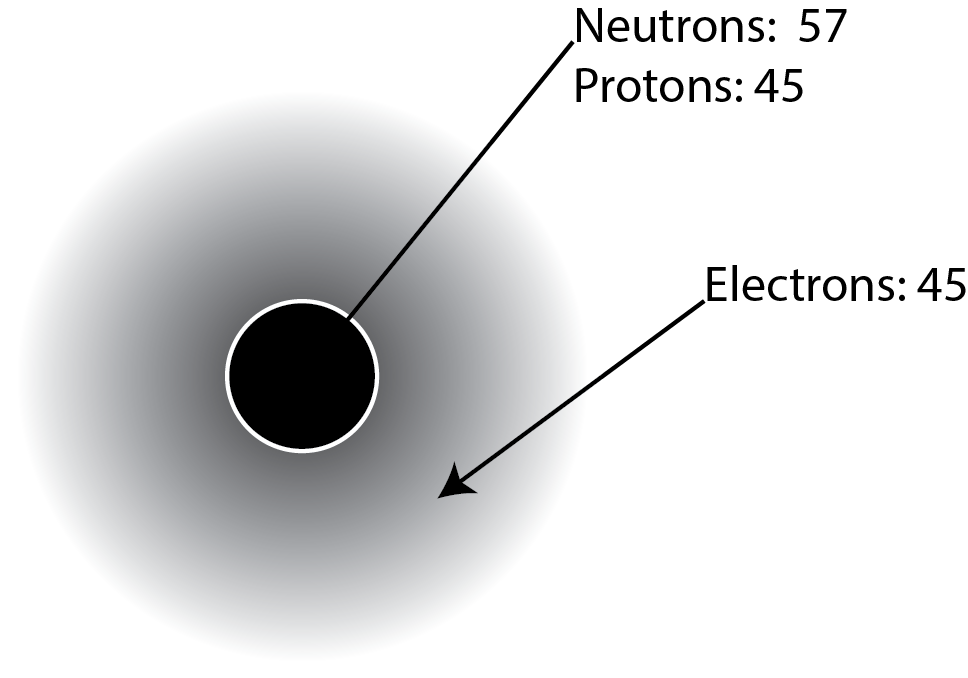
\includegraphics[width=\textwidth]{HW2_102Rh.png}
	\end{subfigure}%
	~
	\begin{subfigure}[b]{0.3\textwidth}
		\centering
		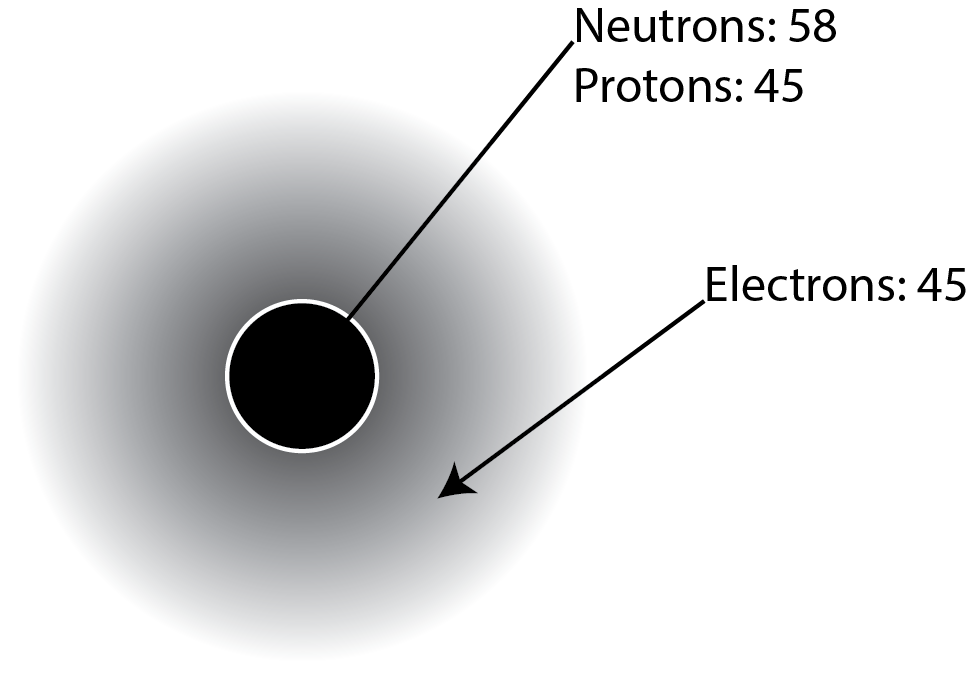
\includegraphics[width=\textwidth]{HW2_103Rh.png}
	\end{subfigure}%
	~
	\begin{subfigure}[b]{0.3\textwidth}
		\centering
		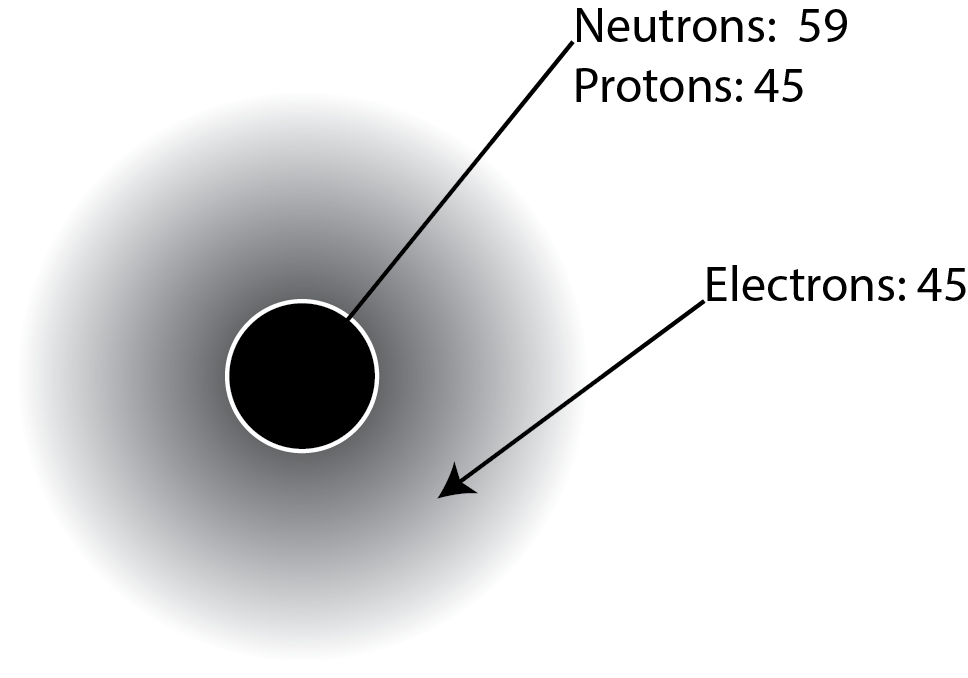
\includegraphics[width=\textwidth]{HW2_104Rh.png}
	\end{subfigure}
	\caption{Isotopes of Z = 45}
	\label{fig:Isotopes}
\end{figure*}

%%%%%%%%%%%%%%%%%%%%%%%%%%%%%%%%%%%%%%%%%%%%%%%%%%%%%%%
\part{g}{Draw three isotones with N = 40}

Isotones are nuclides with the same N, but with different number of protons.
The isotones of N = 40 are shown in Figure ~\ref{fig:Isotones}.
\begin{figure*}[!ht]
	\centering
	\begin{subfigure}[b]{0.3\textwidth}
		\centering
		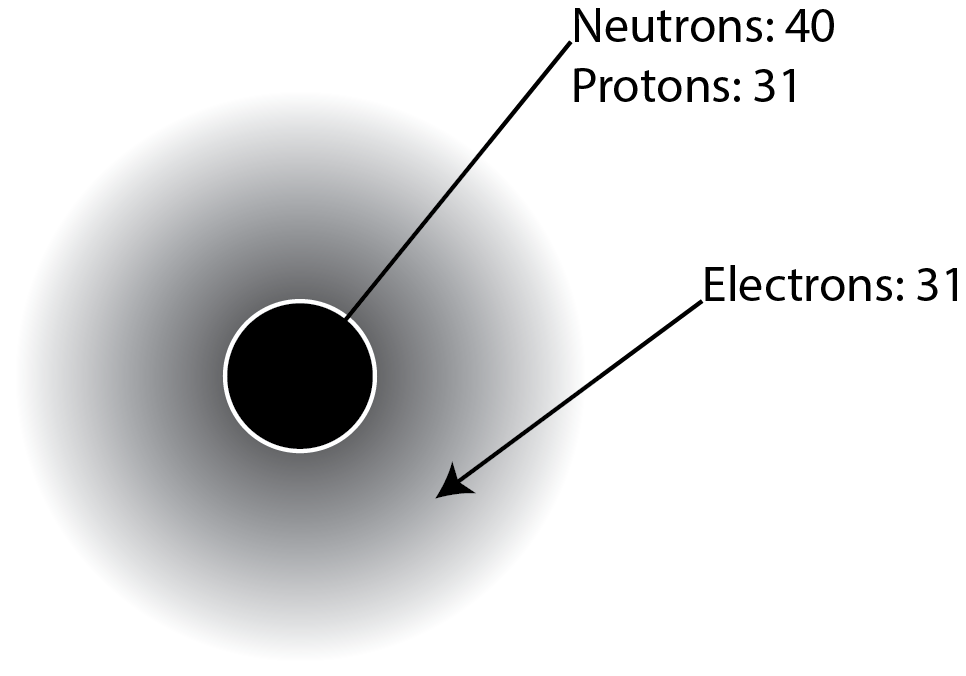
\includegraphics[width=\textwidth]{HW2_71Ga.png}
	\end{subfigure}%
	~
	\begin{subfigure}[b]{0.3\textwidth}
		\centering
		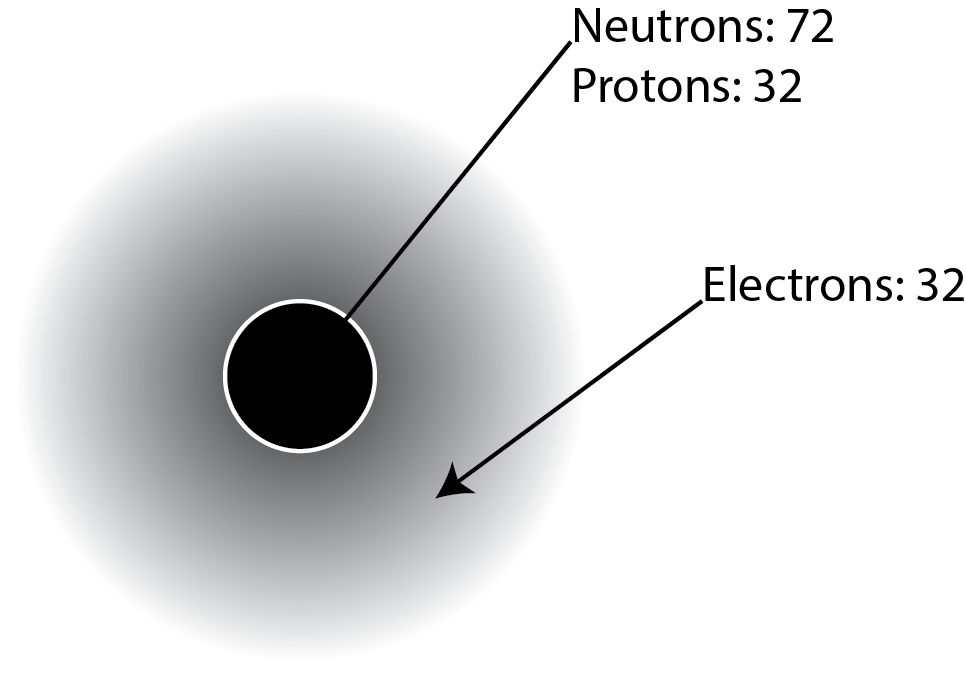
\includegraphics[width=\textwidth]{HW2_72Ge.png}
	\end{subfigure}%
	~
	\begin{subfigure}[b]{0.3\textwidth}
		\centering
		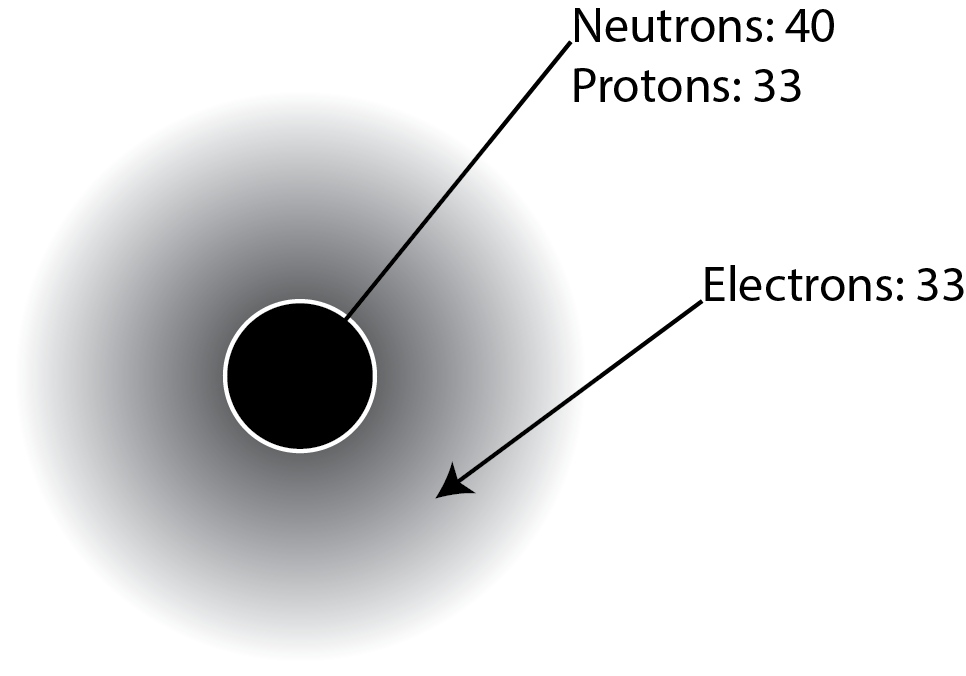
\includegraphics[width=\textwidth]{HW2_73As.png}
	\end{subfigure}
	\caption{Isotones of N = 40}
	\label{fig:Isotones}
\end{figure*}

%%%%%%%%%%%%%%%%%%%%%%%%%%%%%%%%%%%%%%%%%%%%%%%%%%%%%%%
\part{h}{Draw three isobars with A = 69}

Isobars are nuclides with the same A.
The isobars of A = 69 are shown in Figure ~\ref{fig:Isobars}
\begin{figure*}[!ht]
	\centering
	\begin{subfigure}[b]{0.3\textwidth}
		\centering
		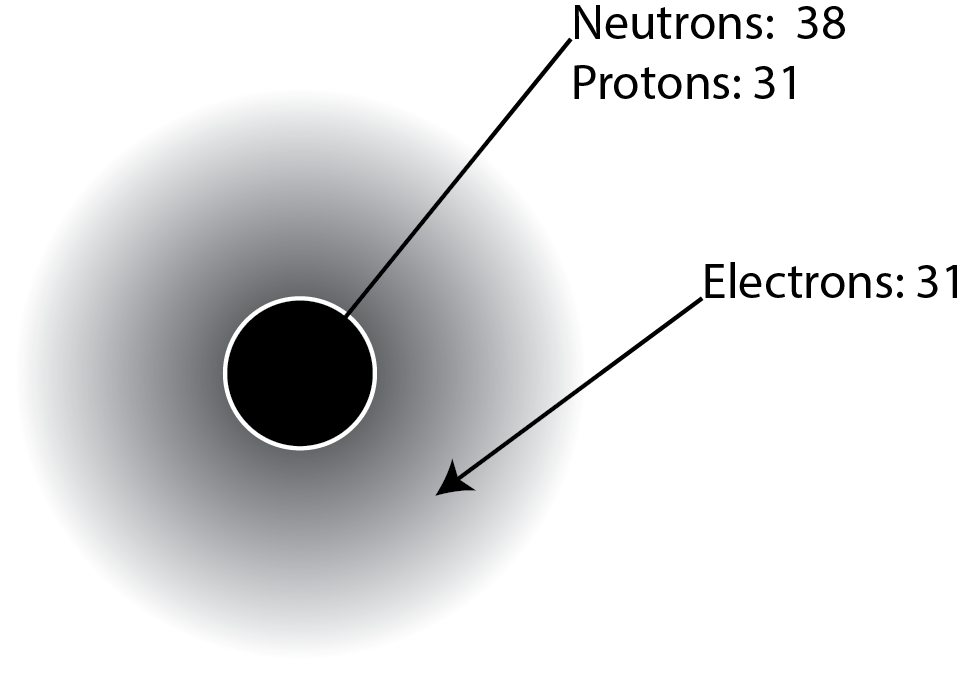
\includegraphics[width=\textwidth]{HW2_69Ga.png}
	\end{subfigure}%
	~
	\begin{subfigure}[b]{0.3\textwidth}
		\centering
		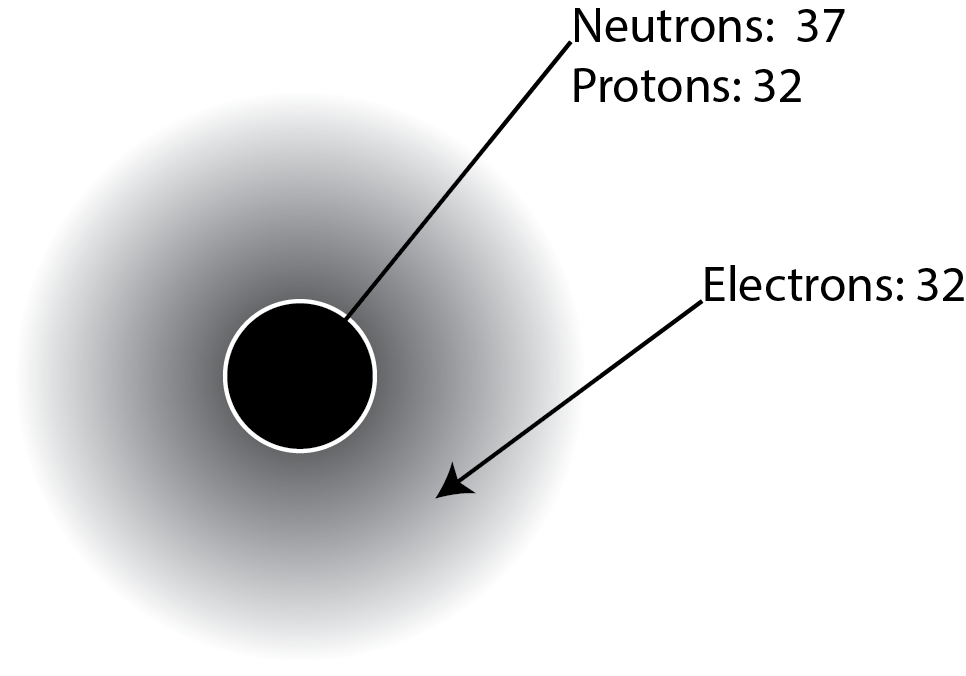
\includegraphics[width=\textwidth]{HW2_69Ge.png}
	\end{subfigure}%
	~
	\begin{subfigure}[b]{0.3\textwidth}
		\centering
		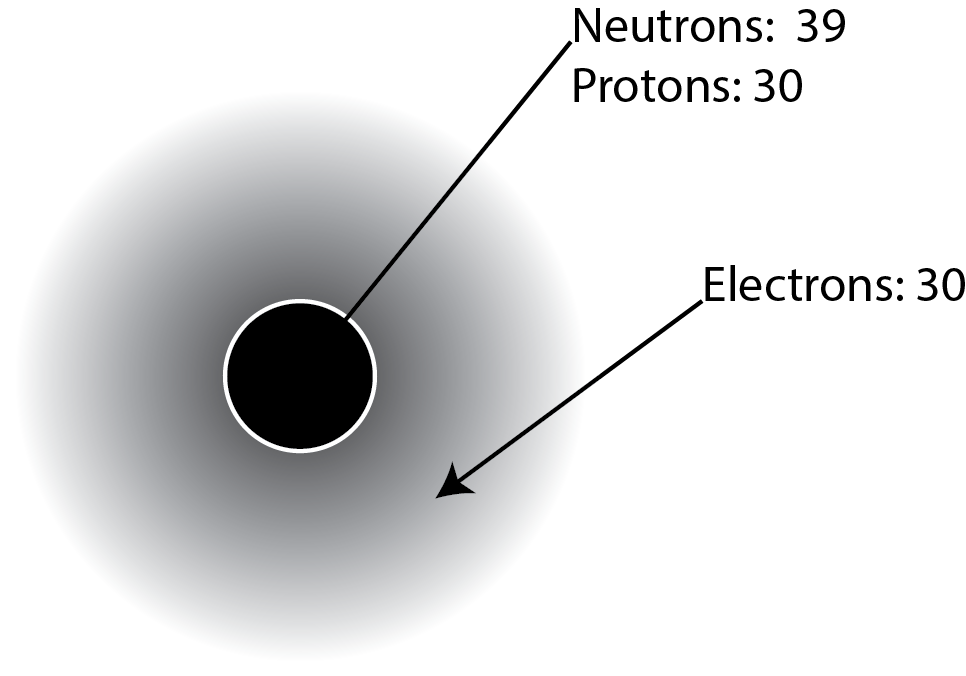
\includegraphics[width=\textwidth]{HW2_69Zn.png}
	\end{subfigure}
	\caption{Isobars of A = 69}
	\label{fig:Isobars}
\end{figure*}

%%%%%%%%%%%%%%%%%%%%%%%%%%%%%%%%%%%%%%%%%%%%%%%%%%%%%%%
\part{g}{Identify the nuclide with $I=0$, the one with $I\ge0$, and the one with a half number I}

\begin{itemize}
	\item Even-even isotopes have $I=0$, therefore \isotope[40]{Ca}
	\item Odd-odd isotopes have an integer spin, therefore \isotope[36]{Cl}
	\item Even-odd isotopes have half integer spin, therefore \isotope[49]{Ti}
\end{itemize}

\question{Advanced Topic}{Extended Periodic Table - Part 2, Binding Energy}

The binding energy per nucleon was investigated using the semi-empirical mass model along with published data.
For each A, Z the semi-empirical mass model was used to calculate the binding energy, with the results shown in the contour plot of Figure ~\ref{fig:BESemiEmperical}.
It is immediately evident why the heavy elements tend to have more isotopes, because their is a large plateau in the 8 MeV per nucleon range.
This plateau ends around a Z of 80, which is around where the elements have a high change of being radioactive.
In addition, the binding energy per nucleon starts to decline, indicating that according the the semi-empirical mass model that there is a finite number of elements\footnote{The coefficients of the semi-empirical mass model are from fitted data, so it probably should not be extrapolated very far}.
The semi-empirical binding energy per nucleon was compared to the published values from the NNDC\footnote{Data from http://www.nndc.bnl.gov/masses/mass.mas03}, and the log error between the two was calculated and shown in Figure ~\ref{fig:BEError}.
In general, there was very good agreement.  However, the real values did not show as much variability as the semi-empirical model. In addition, the semi-empirical model fails to capture the binding energy at very low A and Z, where quantum / shell models would be more accurate.
\begin{figure}[hb]
	\centering
	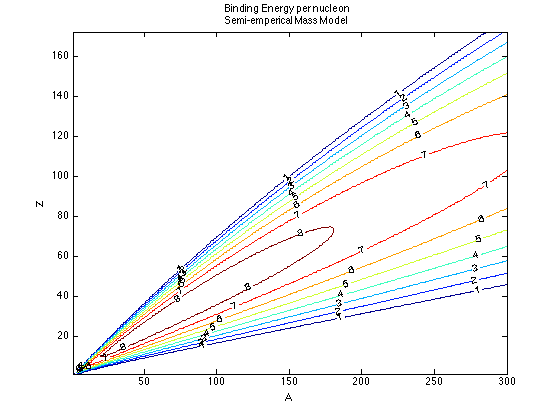
\includegraphics[width=\textwidth]{BEPerNuc_SemiEmp.png}
	\caption{Binding Energy per Nucleon (Semi-empirical Mass Model)}
	\label{fig:BESemiEmperical}
\end{figure}
\begin{figure}[ht]
	\centering
	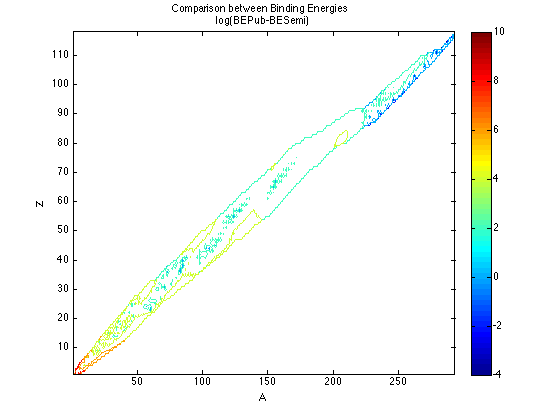
\includegraphics[width=\textwidth]{BEError.png}
	\caption{Binding Energy Error (Log Difference)}
	\label{fig:BEError}
\end{figure}
\end{document}

